\subsection{Denoising a quaternion graph signal via QLMS low-pass filtering}

Let us walk through an example on spectral analysis with real-world data using QGSP. The graph signal will be generated using UK towns' weather data, specifically humidity, atmospheric pressure, temperature and wind speed. The data was fetched from the Open Weather Map API\footnote{The API is accessible, as of August 2022, at the address \url{https://home.openweathermap.org/}.}, in April 20th 2022, at approximately 13:00 GMT. The latitude and longitude values of UK towns originate from the LatLong.Net database\footnote{Accessible, as of August 2022, at the address \url{https://www.latlong.net/category/towns-235-55.html}.}.

\begin{figure}
	\centering
	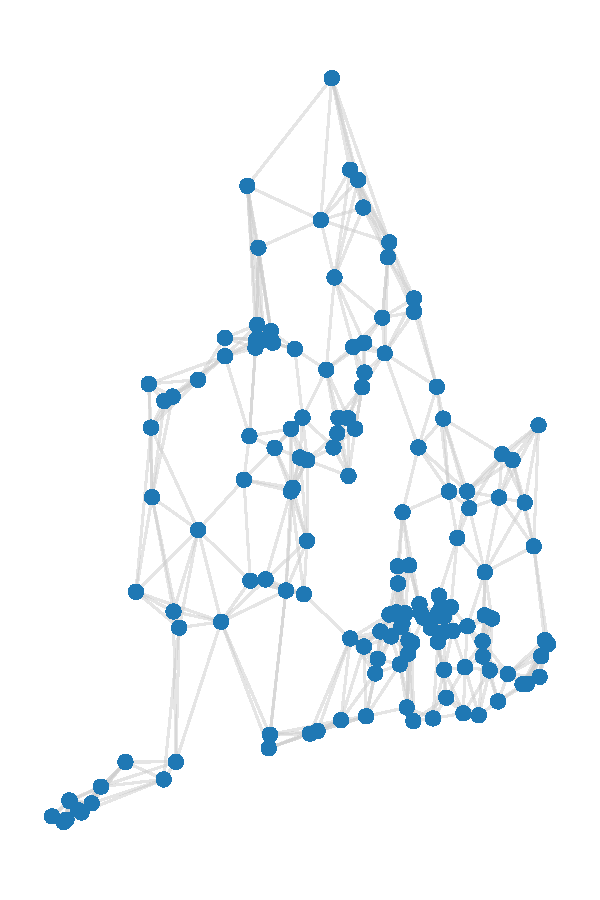
\includegraphics[width=0.3\linewidth]{thesis/Figures/uk_qgsp_graph.pdf}
	\caption{Graph created using the towns in England.}
	\label{fig:uk_graph}
\end{figure}

The graph was created using a nearest-neighbors approach, as in (\ref{eq:weights}), since the nodes possess a clear relation to geographic location. The edge weights were defined using the following steps:
\begin{itemize}[noitemsep]
\item Compute a real-valued nearest-neighbors adjacency matrix based on the latitude and longitude of UK towns (graph nodes), using the ten closest neighbors to each graph node. At this point, the real-valued edge weights correspond to the euclidian distances between nearby towns \textit{i} and \textit{j}, represented by ${d}(i, j)$.
\item For each pair of connected nodes from the real-weighted graph in the previous step, compute the \textbf{absolute difference} in \textit{humidity}, \textit{temperature} and \textit{wind speed}, represented respectively by ${h}(i, j)$, ${t}(i, j)$ and ${w}(i, j)$.
\item For each pair of connected nodes, create the quaternion $q(i, j) = {d}(i, j) + \qi {h}(i, j) + \qj {t}(i, j) + \qk {w}(i, j)$ and set as edge weight the value
\begin{equation}
% \label{eq:}
\mathbf{A}_{i, j} = \exp^{-1} \left(\frac{q}{\theta} \right).
\end{equation}
For the current example, it was chosen $\theta = 0.5$.
\end{itemize}
Figure \ref{fig:uk_graph} depicts a representation of the UK Town Graph, with quaternion-valued edge weights. A total of 177 towns were used, and the reader may find the full dataset at \url{https://github.com/gboaviagem/gspx/blob/main/resources/uk_weather_at_20Apr202213pm.gz}. The first few rows, so it becomes clear how the data is organized, are displayed in Table \ref{tab:02}.

\begin{table}
\center
\captionof{table}{Sample of the dataset containing UK towns' weather data \red{Update!}}
\label{tab:02}
\begin{tabular*}{\textwidth}{c @{\extracolsep{\fill}} cccc}
\toprule
& \textbf{town} & \textbf{latitude} & \textbf{longitude} & \textbf{humidity (\%)} \\
\midrule
1 & Troon, Scotland & 55.540001 & -4.66 & 55\\
2 & St.Asaph, Wales & 53.257999 & -3.442 & 59\\
3 & Stirling, Scotland & 56.1166 & -3.9369 & 53\\
4 & Welling, Bexley, London & 51.4566 & 0.1056 & 39 \\
5 & Bonnybridge, Scotland & 56.003227 & -3.888634 & 50\\
\midrule
\end{tabular*}
\begin{tabular*}{\textwidth}{c @{\extracolsep{\fill}} cccc}
& \textbf{pressure (hPa)} & \textbf{temp (K)} & \textbf{wind speed (m/s)} & \textbf{wind degrees} \\
\midrule
1 & 1018 & 289.19 & 3.6 & 220 \\
2 & 1017 & 288.49 & 3.71 & 99 \\
3 & 1018 & 288.15 & 3.72 & 114 \\
4 & 1014 & 290.09 & 8.23 & 80 \\
5 & 1018 & 288.0 & 3.53 & 106 \\
\bottomrule
\end{tabular*}
\end{table}

% With the quaternion-valued adjacency matrix $\mathbf{A}$ at hand, it was verified that this quaternion graph shift operator (QGSO) was diagonalizable and the direct ($\mathbf{V}^{-1}$) and inverse ($\mathbf{V}$) QGFT matrices were computed. Figure \ref{fig:uk_graph_tv} shows the total variation of the eigenvectors associated with the adjacency matrix eigenvalues.

% \begin{figure}
% 	\centering
% 	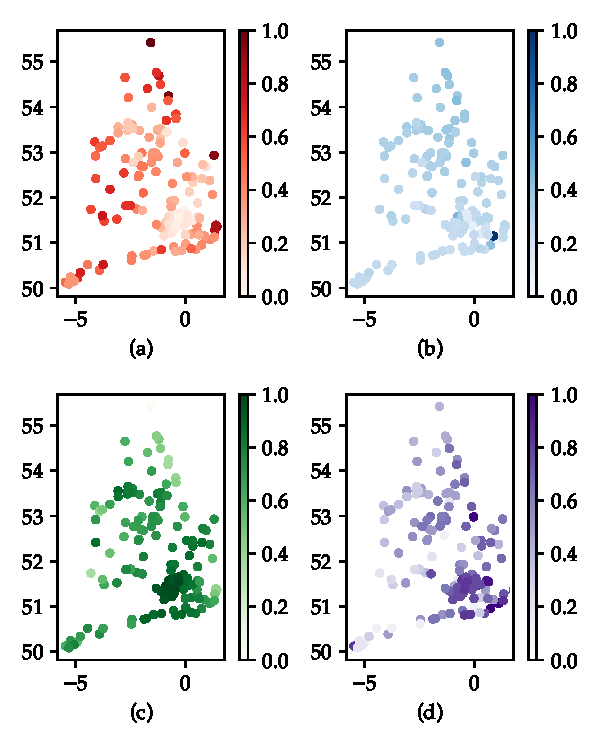
\includegraphics[width=0.6\linewidth]{thesis/Figures/uk_qgsp_sig.pdf}
% 	\caption{Each component of the quaternion graph signal.}
% 	% \label{fig:graph_tv_1}
% \end{figure}

% \begin{figure}
% 	\centering
% 	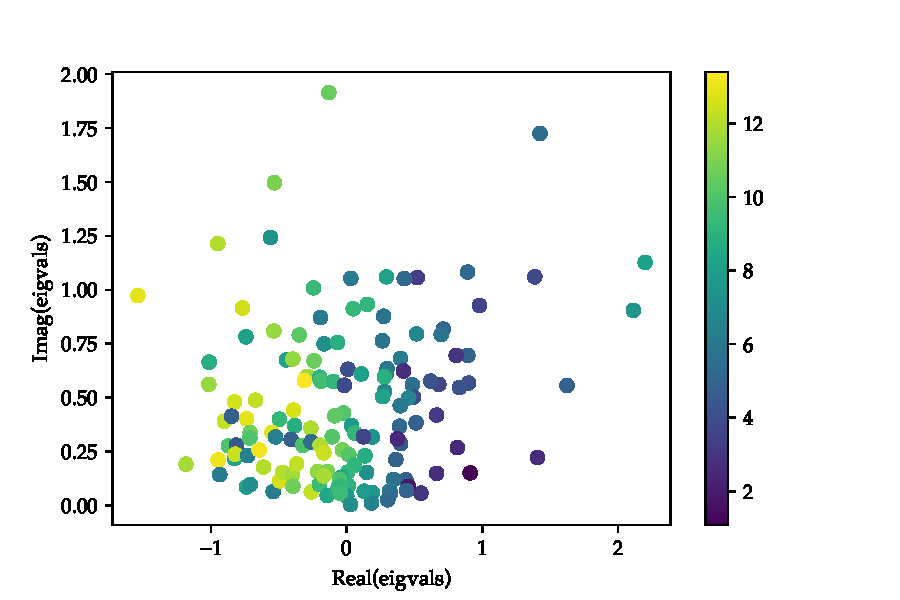
\includegraphics[width=0.6\linewidth]{thesis/Figures/uk_qgsp_tv1.pdf}
% 	\caption{Eigenvalues of the quaternion graph adjacency matrix, shown in the complex plane. The pseudo-colorscale indicates the respective eigenvectors total variation.}
% 	\label{fig:graph_tv_1}
% \end{figure}

% \begin{figure}
% 	\centering
% 	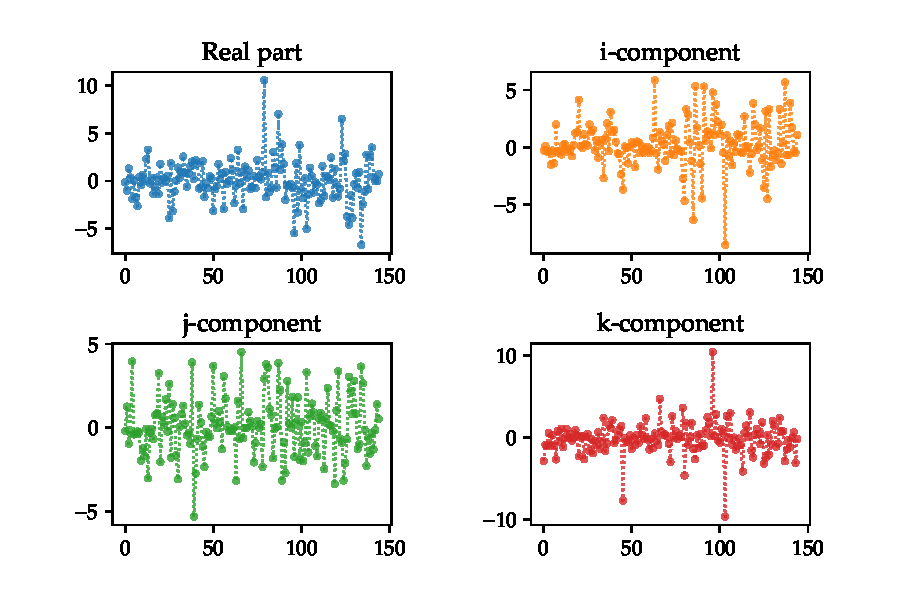
\includegraphics[width=0.6\linewidth]{thesis/Figures/uk_qgsp_spectrumsig_norm1.pdf}
% 	\caption{Eigenvalues of the quaternion graph adjacency matrix, shown in the complex plane. The pseudo-colorscale indicates the respective eigenvectors total variation.}
% 	% \label{fig:graph_tv_1}
% \end{figure}

% \begin{figure}
% 	\centering
% 	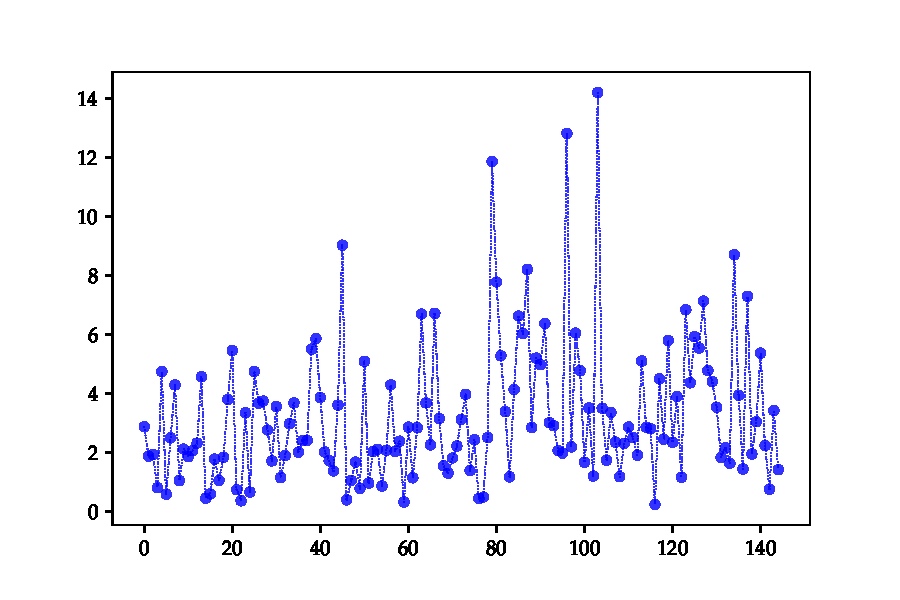
\includegraphics[width=0.6\linewidth]{thesis/Figures/uk_ss1_abs.pdf}
% 	\caption{Eigenvalues of the quaternion graph adjacency matrix, shown in the complex plane. The pseudo-colorscale indicates the respective eigenvectors total variation.}
% 	% \label{fig:graph_tv_1}
% \end{figure}

% \begin{figure}
% 	\centering
% 	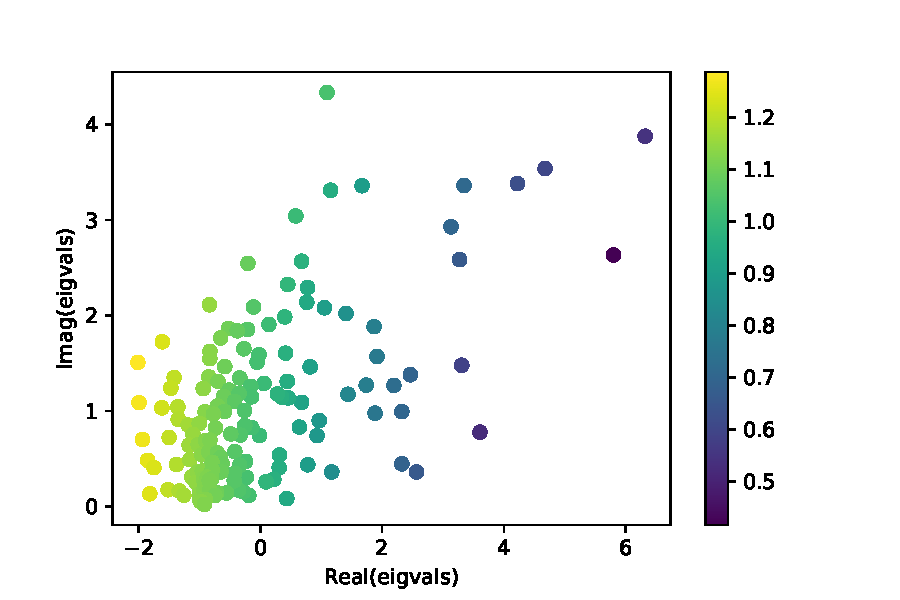
\includegraphics[width=0.6\linewidth]{thesis/Figures/uk_qgsp_tv2.pdf}
% 	\caption{Eigenvalues of the quaternion graph adjacency matrix, shown in the complex plane. The pseudo-colorscale indicates the respective eigenvectors total variation.}
% 	\label{fig:graph_tv_2}
% \end{figure}

% \begin{figure}
% 	\centering
% 	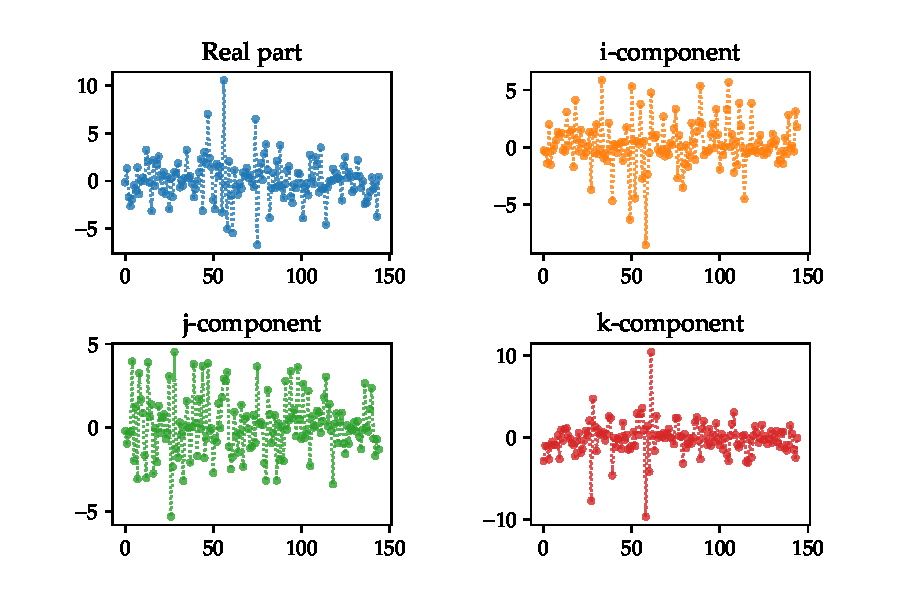
\includegraphics[width=0.6\linewidth]{thesis/Figures/uk_qgsp_spectrumsig_norm2.pdf}
% 	\caption{Eigenvalues of the quaternion graph adjacency matrix, shown in the complex plane. The pseudo-colorscale indicates the respective eigenvectors total variation.}
% 	% \label{fig:graph_tv_1}
% \end{figure}

% \begin{figure}
% 	\centering
% 	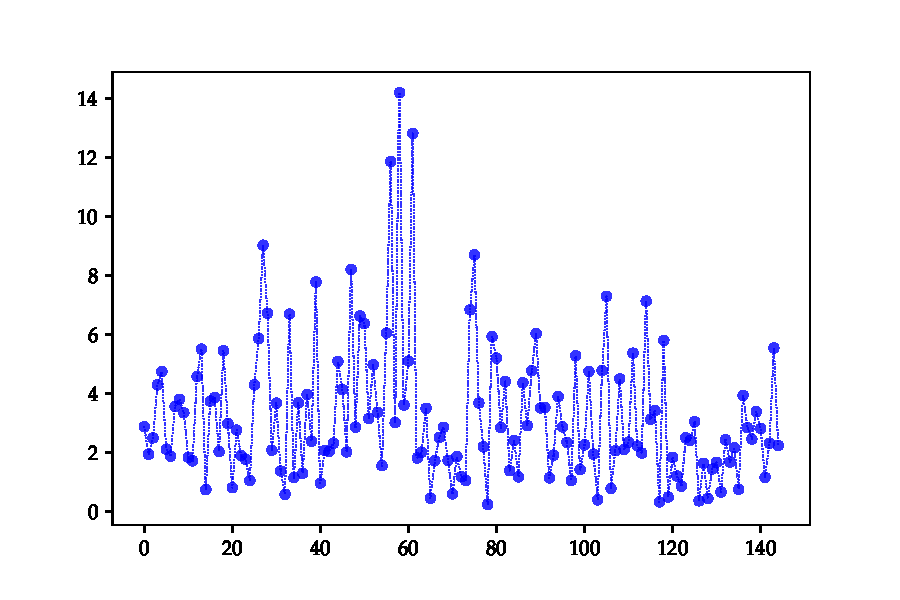
\includegraphics[width=0.6\linewidth]{thesis/Figures/uk_ss2_abs.pdf}
% 	\caption{Eigenvalues of the quaternion graph adjacency matrix, shown in the complex plane. The pseudo-colorscale indicates the respective eigenvectors total variation.}
% 	% \label{fig:graph_tv_1}
% \end{figure}

One may define a quaternion graph signal as being composed by the four last columns of weather data in UK towns (see Table \ref{tab:02}). That is, each sample corresponds to the quaternion with components $(1, \qi, \qj, \qk)$ respectively equal to humidity, pressure, temperature and wind speed in the given town. The scale disparity between components is removed by scaling each column to be within range $[0, 1]$. A way of visualizing the graph signal is to plot each quaternion dimension separately, as done in Figure \ref{fig:uk_qgsp_graphsig}.

\begin{figure}
	\centering
	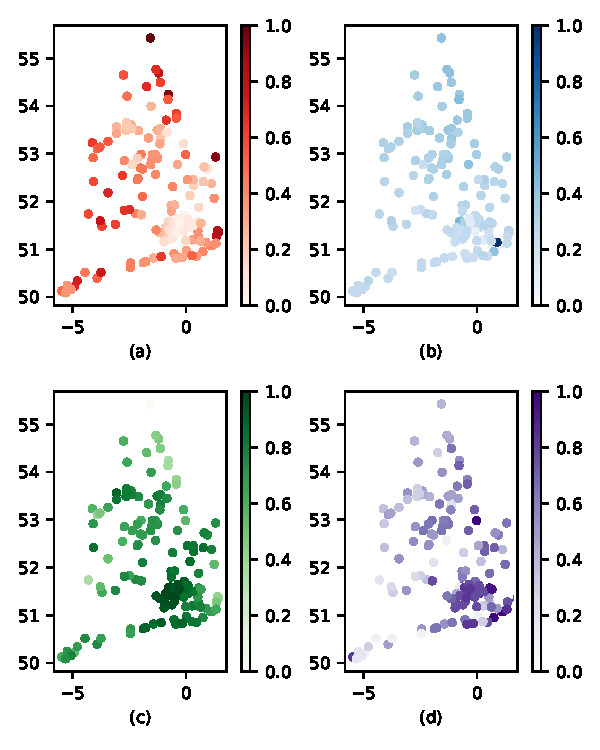
\includegraphics[width=0.5\linewidth]{thesis/Figures/uk_signal.pdf}
	\caption{Quaternion graph signal, visualized in the vertex domain. The panels (a) to (d) depict, respectively, the real, $\qi$, $\qj$ and $\qk$ components of each quaternion-valued sample.}
	\label{fig:uk_qgsp_graphsig}
\end{figure}

\red{Rewrite this paragraph. Comment on the eigenvectors total variation, in Figure \ref{fig:uk_qgft_tv1}} Complementary to the vertex-domain visualization is the spectrum of the signal. This is obtained by the direct QGFT,
\begin{equation}
% \label{}
\widehat{\mathbf{s}} = \mathbf{V}^{-1} \mathbf{s},
\end{equation}
and the signal frequency components are shown in Figure \ref{fig:uk_qgsp_spectrumsig}.

\begin{figure}
	\centering
	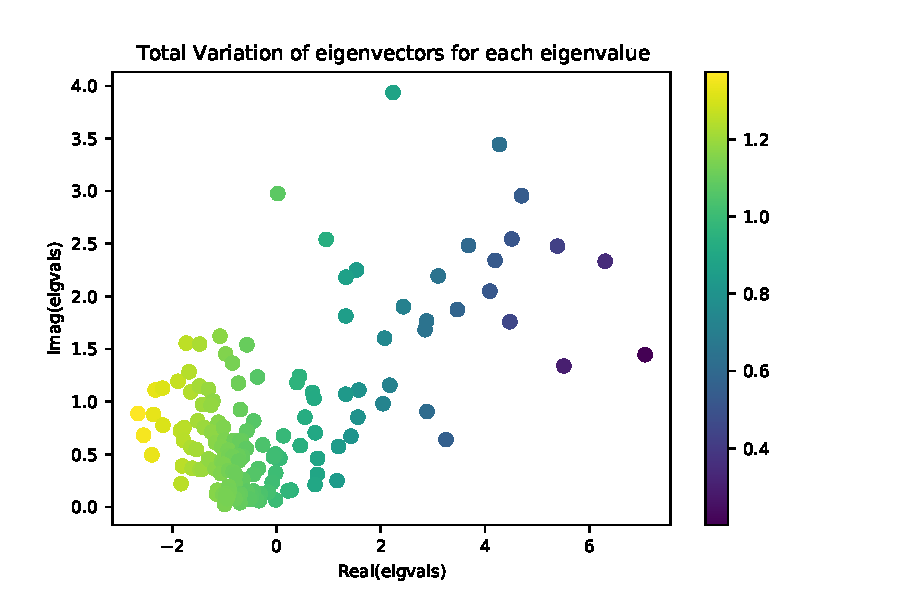
\includegraphics[width=0.7\linewidth]{thesis/Figures/uk_qgft_tv1.pdf}
	\caption{Graph eigenvectors total variation using $\ell_1$-norm.}
	\label{fig:uk_qgft_tv1}
\end{figure}

\begin{figure}
	\centering
	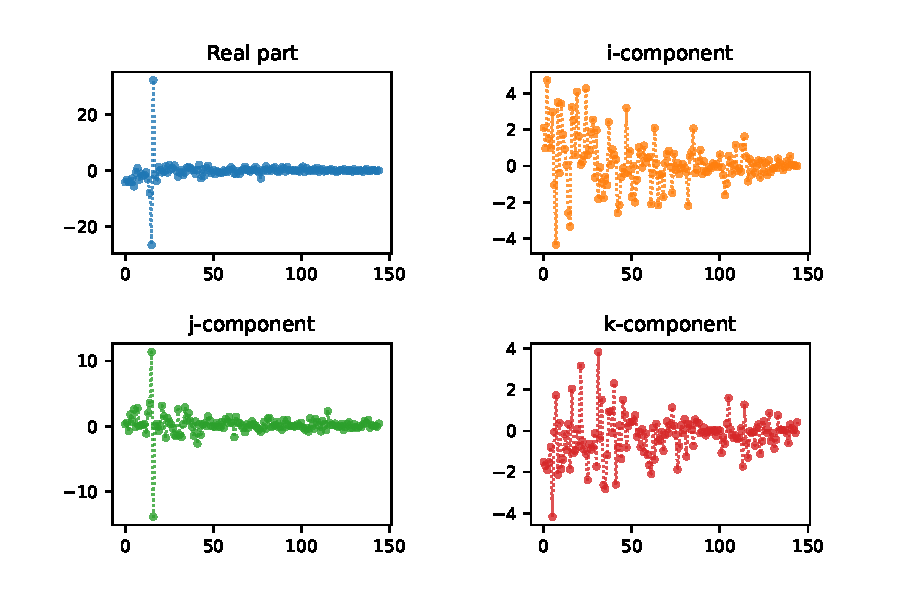
\includegraphics[width=0.7\linewidth]{thesis/Figures/uk_qgft_spectrumsig.pdf}
	\caption{Spectrum of the graph signal in the symmetric graph.}
	\label{fig:uk_qgsp_spectrumsig}
\end{figure}


\begin{figure}
	\centering
	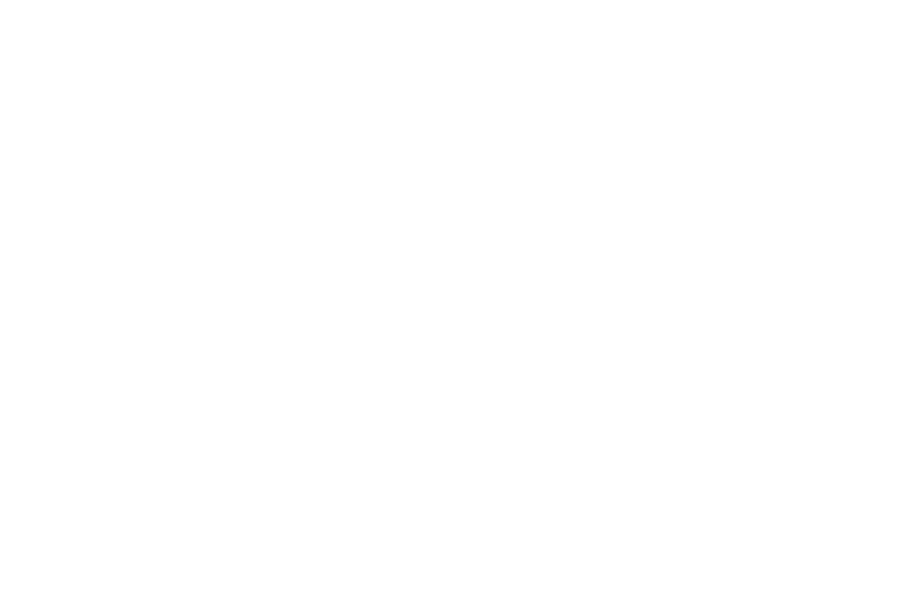
\includegraphics[width=0.7\linewidth]{thesis/Figures/cost_vs_iterations.pdf}
	\caption{.}
	\label{fig:cost_vs_iterations}
\end{figure}

\begin{figure}
	\centering
	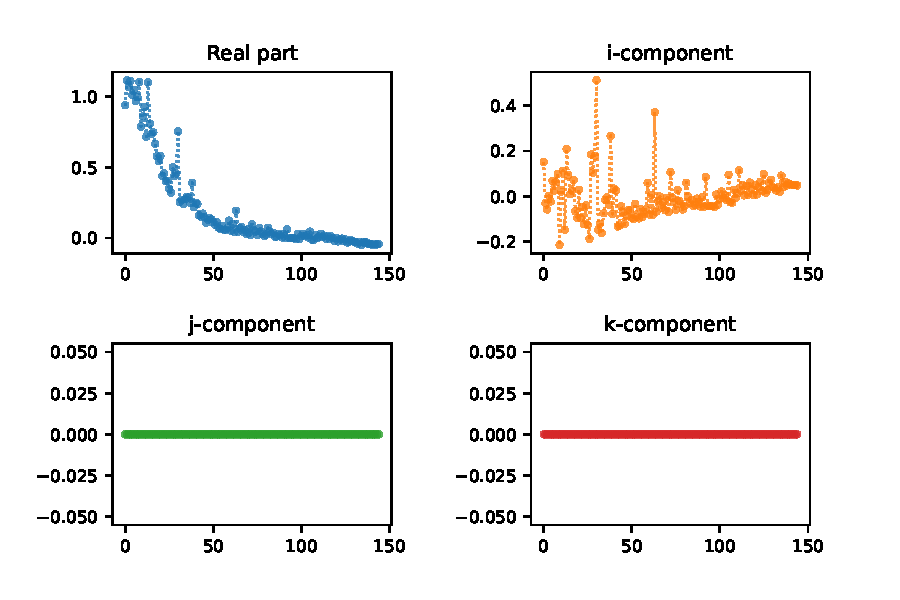
\includegraphics[width=0.7\linewidth]{thesis/Figures/qlms_filter.pdf}
	\caption{.}
	\label{fig:qlms_filter}
\end{figure}

\begin{figure}
	\centering
	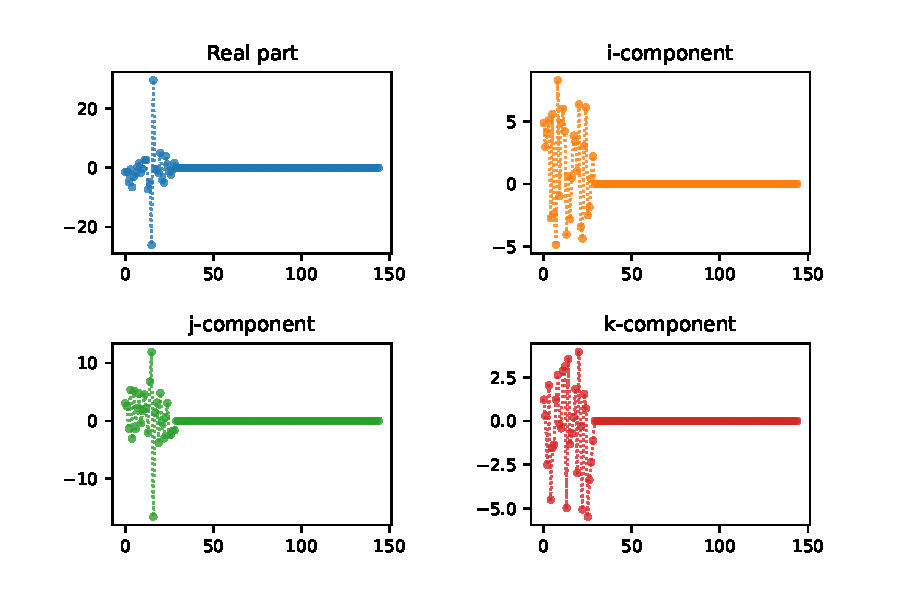
\includegraphics[width=0.7\linewidth]{thesis/Figures/ideal_filter_output.pdf}
	\caption{.}
	\label{fig:ideal_filter_output}
\end{figure}

\begin{figure}
	\centering
	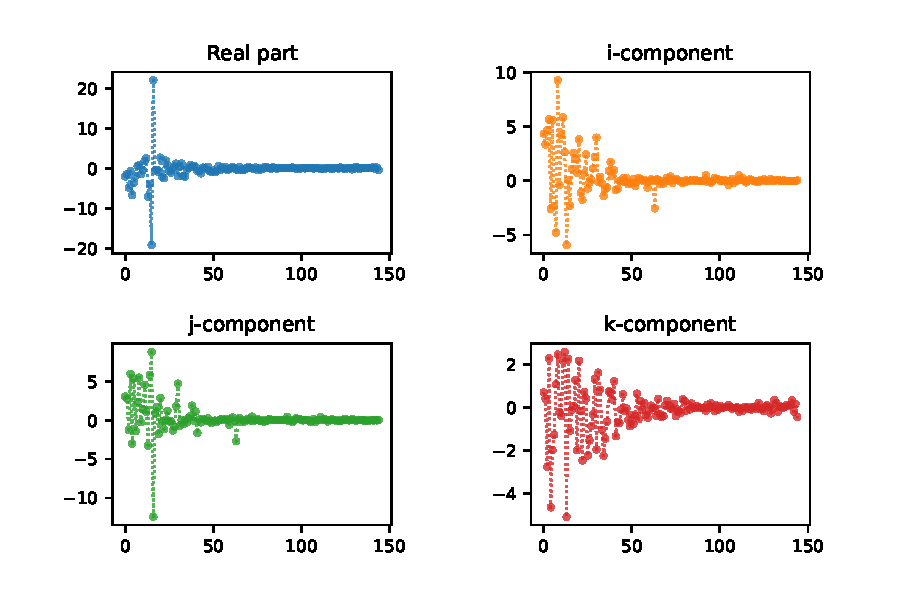
\includegraphics[width=0.7\linewidth]{thesis/Figures/qlms_filter_output.pdf}
	\caption{.}
	\label{fig:qlms_filter_output}
\end{figure}

\subsubsection{Comparison between signal smoothness in symmetric and Hermitian graphs}
\red{Draw a comment here about the drawback of using Hermitian graphs (which we know have always diagonalizable adjacency matrices): they do not capture the expected relation between signal samples when the domain represents undirected influences.}

\red{Also comment the difference in calculations made to create the symmetric and Hermitian graphs.}

Figure \ref{fig:uk_qgft_spectrumsig_hermitian}

\begin{figure}
	\centering
	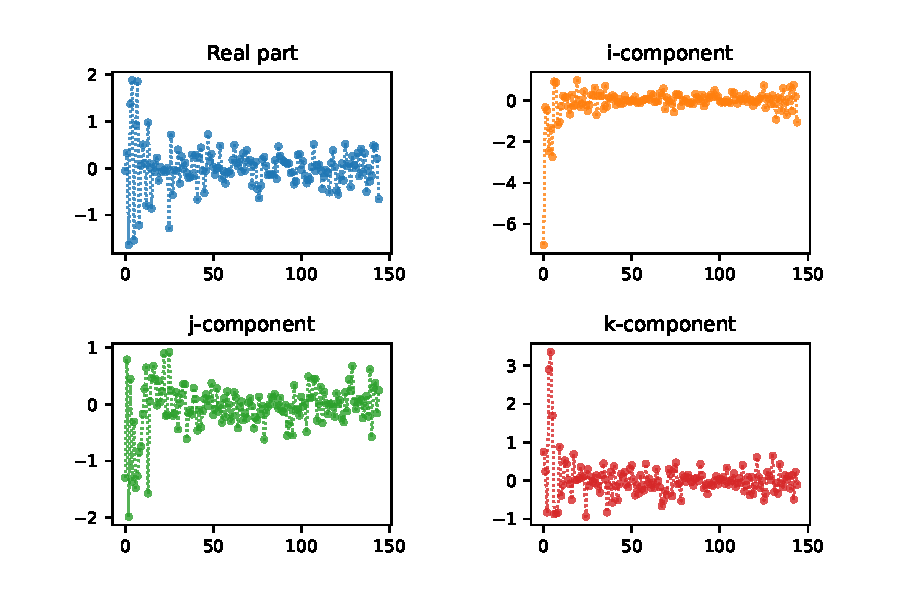
\includegraphics[width=0.7\linewidth]{thesis/Figures/uk_qgft_spectrumsig_hermitian.pdf}
	\caption{Spectrum of the graph signal in the Hermitian graph.}
	\label{fig:uk_qgft_spectrumsig_hermitian}
\end{figure}